% Instructions to change to html version:
% Comment out:
%  minipage, multicols,columnbreak, mathbf, hrule
% Replace all: \begin{minipage}% \end{minipage} %\begin{multicols}  %\end{multicols} 
% \columnbreak
 %	%% \begin{framed} %\end{framed} %%\hrule
% Replace \mathbf with	\boldsymbol
% Replace $$ with \[ or \]and $ with \( or \)
% Enclose graphics in figure environments and add captions
% 			search \includegraphics
% Re-tag \df environments as sections, subsections, etc.
% Command Line Code to Create html version:
%First: pdflatex -shell-escape filename.tex                                   
%Second, for each figure: inkscape "filename-figure1.pdf" -o "filename-figure1.png"
% Third: htlatex filename.tex "ht5mjlatex.cfg, charset=utf-8" " -cunihtf -utf8"

\documentclass[10pt]{article}

%\usepackage{tikz, pgf,pgfplots,wasysym,array}
%\usepackage{wasysym,array}

\usepackage{amsmath,amssymb}
\usepackage[hidelinks]{hyperref}

\ifdefined\HCode
  \def\pgfsysdriver{pgfsys-tex4ht-updated.def}
\fi 
%\ifdefined\HCode
%  \def\pgfsysdriver{pgfsys-dvisvgm4ht.def}
%\fi 
\usepackage{tikz}
\usetikzlibrary{calc,decorations.markings,arrows}
\usepackage{pgfplots}

\pgfplotsset{compat=1.12}
\usepackage{myexternalize}
\usetikzlibrary{calc,decorations.markings,arrows}
\usepackage{framed}
\usepackage[none]{hyphenat}

\input{../../../common/1336_header_test.tex}
\begin{document}

\newcommand{\an}{\lbrace a_n \rbrace}
\newcommand{\Sum}{\sum_{n=1}^\infty }

\everymath{\displaystyle}

\renewcommand{\myTitle}{MATH 1336: Calculus III}

\renewcommand{\mySubTitle}{Section 5.5:  Alternating Series \& Absolute Convergence }
%~\hfill Name: \underline{~~~~~~~~~~~~~~~~~~~~~~~~~~~~~~~~~~~~~~~~~~~~~~~}

\lectTitle{\vspace*{-.5in}\myTitle}{\vspace*{.1in}\mySubTitle \vspace*{-.2in}}




%\hspace*{-.8in}%\begin{minipage}{1.25\textwidth}

\setlength{\columnseprule}{.4pt}
\setlength{\columnsep}{3em}

%\begin{framed}
\df{\textcolor{sblack}{Sections 5.5 \& 5.6 - More Series Tests!: }}~\\
In these sections, we'll learn tests that can be applied to series that may have some negative terms.\\

%\hrule
\vspace*{.1in}

%\begin{multicols}{2}



\df{\textcolor{sblack}{Alternating Series Test (AST):}}~\\
If an alternating series can be written in one of the  following forms:\\ ~\\
\(\Sum (-1)^{n+1}\ b_n = b_1 - b_2 + b_3 - b_4 + b_5 - b_6+ \ldots = \Sum (-1)^{n-1}\ b_n\)\\~\\~\\
-OR-\\ ~\\
\(\Sum (-1)^{n}\ b_n = -b_1 + b_2 - b_3 + b_4 - b_5 + b_6- \ldots\)\\~\\~\\
and satisfies both of the conditions listed below, then the series is convergent.
% \begin{multicols}{2}
 \begin{enumerate}[(i)] 
 \item \(0<b_{n+1} \leq b_n\)
 \item \(\lim_{n\rightarrow \infty} b_n = 0\)
 \end{enumerate} 
 %%\end{multicols}%\( \\~\\~\\
 
 \vspace*{.5in}
 %\columnbreak

\df{\textcolor{sblack}{Alternating Series Estimation/Remainder Theorem:}}~\\
If \(S\)  is the sum of a convergent alternating series
\[
\Sum (-1)^{n+1}\ b_n  \qquad \text{-OR-} \qquad \Sum (-1)^{n}\ b_n ,
\]
 then 
\[
|R_N| = |S - S_N| \leq b_{N+1}
\]
~\\
\begin{figure}[!h]
\centering
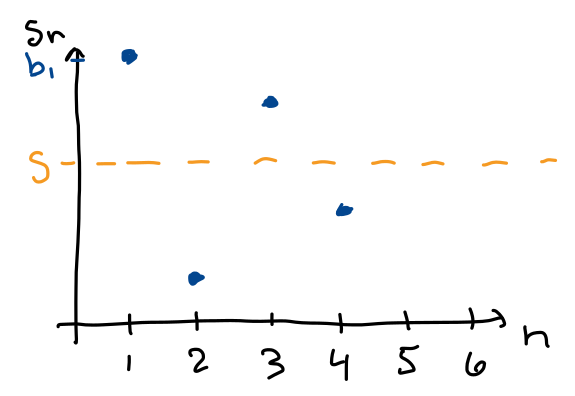
\includegraphics[width=.75\columnwidth]{Ch8s4-ASET.png}
\caption{Illustration of a convergent alternating series to demonstrate the Alternating Series Estimation Theorem.}
\end{figure}
%\end{multicols}

%\hrule
\vspace*{.1in}

\df{\textcolor{sblack}{Absolute \& Conditional Convergence:}}
%\begin{multicols}{2}
A series \(\sum a_n\) is called \textbf{absolutely convergent} if the series \(\sum |a_n|\) is convergent.\\~\\

A series \(\sum a_n\) is called \textbf{conditionally convergent} if it is convergent, but \textit{not} absolutely convergent.

%\columnbreak

\textbf{Theorem 5.15:}\\
If a series \(\sum |a_n|\) converges, then \(\sum a_n\) converges.

%\end{multicols}


%\end{framed}

%\end{minipage}

\pagebreak

\section*{Examples:}
 %Determine the convergence behavior of the following series:
\begin{enumerate}[{Example} 1:]



\item Use the AST to show that the Alternating Harmonic Series converges.
\[\Sum \frac{(-1)^{n+1}}{n}\]

\vfill

\hspace*{-.75in} \textit{Follow-up Question:} How many terms would we need to use to obtain an estimate for the sum of the series that is within \(0.01\) of the exact value?

\vfill
%\pagebreak

\item Determine the convergence behavior of the following series.\\
\( \qquad
\Sum \frac{(-1)^n 5n}{6n-2}
\)


\vfill

\pagebreak

\item Let's determine if the following series is absolutely convergent, conditionally convergent, or divergent.\\%  (Problem 3 from 8.3, Part 2!)\\
\(\qquad\Sum \frac{\sin(n)}{n^2}\) %\label{prob3}
%Absolutely Convergent


\vfill

\item Apply the Alternating Series Test to the following series:\\
%%\begin{enumerate}[(a)]
%\item \( \qquad  \sum_{n=2}^\infty \frac{(-1)^n}{n\ (\ln n)^2}\)
%\item 
\( \qquad  \Sum	\frac{(-1)^{n+1}}{2^{n}}\)\label{example1b}
%\end{enumerate}
%\end{multicols}
\vfill

\item Find an upper bound on the error from using only the first 5 terms of the series in Example \ref{example1b} to approximate the sum of the series. 

\vfill




\end{enumerate}

\pagebreak

\section*{Problems for Group Work:}
\textbf{Be sure to fully justify your reasoning as a part of your solutions.}\\
 The answers are upside-down on the bottom of this page.

%\begin{framed}
For Problems \ref{prob1}-\ref{prob4}, determine whether the series is absolutely convergent, conditionally convergent, or divergent.
%\end{framed}

\begin{enumerate}

%\begin{multicols}{2}

\item \(\Sum \frac{(-1)^{n+1}}{n^{2/3}}\) \label{prob1}
%Conditionally Convergent,
\vspace*{2.5in}
%\vspace*{1.75in}

\item \(\Sum \frac{\cos(n\pi) }{n^3}\) \label{prob2}
%Absolutely Convergent,
\vspace*{2.5in}
%\vspace*{1.75in}



\item \(\Sum \frac{(-1)^{n-1}}{1+\frac{1}{n}}\) \label{prob3}
%Divergent
\vspace*{2.5in}
%\vspace*{1.75in}

\item \(\Sum \frac{1}{5^n-3^n}\) \label{prob4}
%Converge
\vspace*{2.5in}
%\vspace*{1.75in}

%\end{multicols}

\end{enumerate}

\vfill

\rotatebox{180}{
%\begin{minipage}{\textwidth}
\underline{Answers:}\\
\textbf{Problem \ref{prob1}:} Conditionally Convergent,
\textbf{Problem \ref{prob2}:} Absolutely Convergent,\\
\textbf{Problem \ref{prob3}:} Divergent,
\textbf{Problem \ref{prob4}:} Absolutely Convergent

%\end{minipage}
}

\end{document}
